\documentclass[]{article}

\usepackage[utf8]{inputenc}
\usepackage{amsmath}
\usepackage{amssymb}
\usepackage{amsthm}
\usepackage{amsfonts}
\usepackage{mathtools}
\usepackage[margin=1.7cm]{geometry}
\usepackage[most]{tcolorbox}
\usepackage{graphicx}
\usepackage{capt-of}
\usepackage{adjustbox}
\usepackage{listings}
\usepackage{cleveref}
\usepackage{siunitx}
\usepackage{subcaption}
\usepackage{siunitx}
\usepackage{biblatex}
\addbibresource{sample.bib}
\usepackage[section]{placeins}
\usepackage{float}




% Section numbering %
\renewcommand\thesection{Assignment \arabic{section}}
\renewcommand\thesubsection{\arabic{subsection}}

% Proofs
\newcommand\TombStone{\rule{.5em}{.5em}} % The tombest stone
\renewcommand\qedsymbol{\TombStone}
\renewcommand{\proofname}{Proof.} % Nice proof

\title{Interactive Multiple Model Probability Data Association Filter}
\author{Håvard Mellby \& Sigurd Totland}


\begin{document}
\maketitle

\newpage
\section{}

\subsection{IMM-PDAF}
\subsubsection{IMM}
The behaviour of the targets we want to model might change over time, and any single (reasonably simple) model might not cover all situations. A better approach might be to combine multiple simple models with each model describing a subset of the system's behaviour. In our case we want to model a boat that is either moving straight forward or turning. We can then use an \textit{interactive multiple models} (IMM) approach to combine a CT (Constant Turn) and a CV (Constant Velocity) model. The IMM will weigh the different models based on how well they describe the current state (using the likelihood of the model being the correct one).

\subsubsection{PDAF}
No sensor is perfect and radars are no exception. The radar outputs a lot of measurements which may or may not originate from our target. To solve this we use a \texttt{probability data association filter} to associate measurements with our target and weigh them according to their likelihood of originating from our target.

We can combine the IMM and PDAF to develop the \texttt{interactive multiple models probability data association filter} to track a moving boat using radar detections.

\subsubsection{Implementation}
A normal IMM filter was developed according to chapter 6 in \cite{edmund} and was initialized with a CT and a CV EKF model. Most of the IMM-PDAF implementation is equal to the PDAF implementation described in chapter 7 in \cite{edmund} using the IMM as the model. There are however one difference that we should emphasize.

When updating the IMM conditional on each possible measurement association we get a new mixture model from the IMM with $M$ components. The total mixture model for the IMM-PDAF after one iteration (assuming single gaussian input) is therefore a mixture model with $(N+1)M$ components where $N$ is the number of gated measurements and $M$ is the number of models. This will again continue to grow for each timestep as new measurements will create additional components.

We therefore want to reduce the number of components by conditioning the association probabilities on the mode probabilities. Further we reduce the mixture for each mode to a single gaussian component using equations (6.18) and (6.20) from \cite{edmund}. The association probabilities conditioned on the mode are used as weights.




\subsection{Tune the IMM-PDAF to the given simulated data}

We initialized the filter using the values from previous excercises which we knew worked well. We then modified the \textit{simulate\_atc\_track.m} script to allow us to generate pure CV and CT tracks and used those to tune the corresponding CV/CT PDAF models, using the NEES $95 \%$ confidence interval (CI) and common sense as metrics. Multiple simulated tracks were used for each model to increase robustness. The measurement noise $r$,clutter intensity $\lambda$, the detection probability $P_D$ and the gate size should be independent of modes, so they were tuned and balanced between the two models. The clutter rate $\lambda$ can be interpreted as the number of false detections per cubic meter and it is therefore reasonable for this number to be quite low. The process noise for CV $q_{cv}$ and CT $q_{ct}$ were tuned individually using their correspondig models. For IMM PDAF tuning we created a custom plot function which allowed us to plot the tracked path in colors corresponding to the mode probability (see \cref{fig:task22_modeprob}). We then tuned the IMM Markov Matrix $PI$ so that the CV model was used during constant velocity sections of the track, and the CT models during the turns (fig \ref{fig:task22_modeprob_tuned}). $q_{cv}$ and $q_{ct}$ does affect the mode probabilities, i.e we risk always preferring one model if the process noises are not balanced (see fig \ref{fig:task22_modeprob_highcv} where $q_{cv}$ is big compared to $q_{ct}$). Our finished tuning works well and seems to balance the two models well. The NEES is mostly within the $95\%$ CI as can be seen in \cref{fig:task22_NEES}. The estimation error, as shown in \cref{fig:task22_tracking_error}, is also quite small and well within what we consider acceptable limits.

\begin{tcolorbox}[ams align, title={Tuning for IMM-PDAF in simulated dataset}]
        r &= 5 & \lambda &= 10^{-4} \label{eq:imm-sim-tuning1} \\
        P_D &= 0.95 & \texttt{gateSize} &= 5^2 \label{eq:imm-sim-tuning2} \\
        q_{cv} &= 0.0078  & q_{ct} &= \begin{bmatrix}0.02 & 0.0005\end{bmatrix} \label{eq:imm-sim-tuning3} \\
        PI &= \begin{bmatrix}0.90 & 0.05 \\ 0.10 & 0.95\end{bmatrix} \label{eq:imm-sim-tuning4}
\end{tcolorbox}

\begin{figure}
    \centering
    \hspace*{-2cm}\begin{adjustbox}{minipage=0.8\linewidth, scale=1}
        \begin{subfigure}{.5\textwidth}
            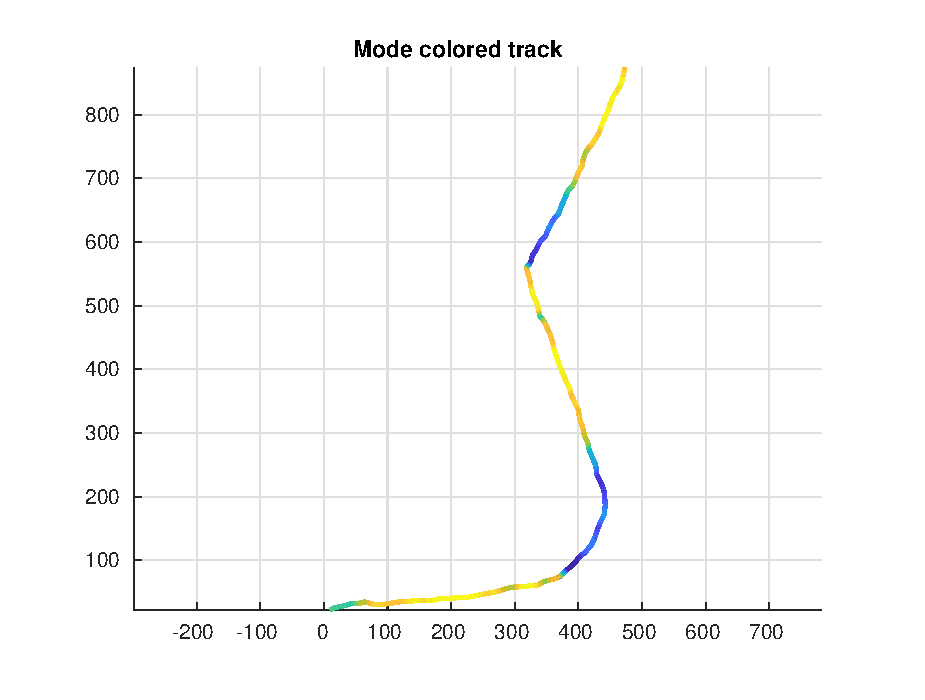
\includegraphics[width=\linewidth]{plots/task22_modeprob.eps} 
            \caption{Our tuning}
            \label{fig:task22_modeprob_tuned}
        \end{subfigure}
        \begin{subfigure}{.5\textwidth}
            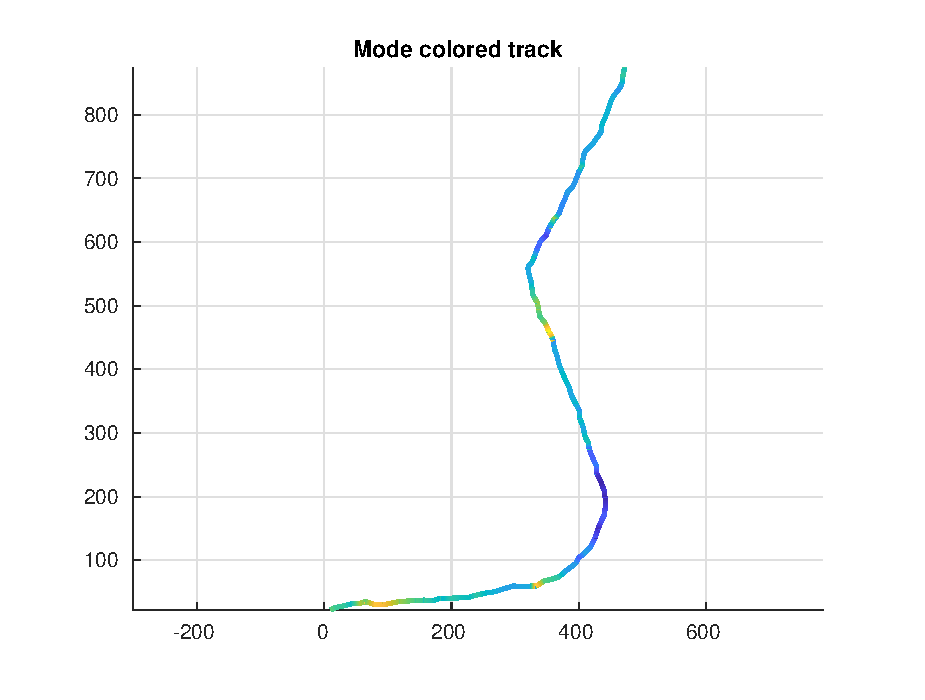
\includegraphics[width=\linewidth]{plots/task22_modeprob_highcv.eps} 
            \caption{$q_{cv}$ and $q_{ct}$ not in balance}
            \label{fig:task22_modeprob_highcv}
        \end{subfigure}
    \end{adjustbox}
        \caption{Mode probability plot: Yellow = CV, Blue = CT}
        \label{fig:task22_modeprob}
\end{figure}

\begin{figure}
    \centering
    \hspace*{-2cm}\begin{adjustbox}{minipage=0.8\linewidth, scale=1}
        \begin{subfigure}{.5\textwidth}
            \includegraphics[width=\linewidth]{plots/a1/task2/a1_task2_error.eps} 
            \caption{Tracking error}
            \label{fig:task22_tracking_error}
        \end{subfigure}
        \begin{subfigure}{.5\textwidth}
            \includegraphics[width=\linewidth]{plots/a1/task2/a1_task2_NEES.eps} 
            \caption{NEES}
            \label{fig:task22_NEES}
        \end{subfigure}
    \end{adjustbox}
        \caption{Tracking performance when using simulated data}
\end{figure}
\subsection{IMM-PDAF on the real data set "Joyroide"}

\subsection{Discussion}
\subsubsection{Balancing Consistency and Tracking Error}
When tuning we want to achieve as good tracking as possible, but we also want the filter to be consistent. An overly confident filter will not fuse measurments that conflict with the prediction (i.e losing track), while an uncertian filter will struggle to aquire a track at all. The filter will not always have perfect track, but it is important that the "confidence" of the filter scales well with how good the track actually is.
When tuning we therefore use the NEES CI as a metric for how confident the filter is compared to how well the filter tracks the target. It should be noted that calculating NEES for a single dataset is not ideal, and we should run several iterations (Monte Carlo simulations) of this to test how well the filter generalizes.

\subsubsection{IMM-PDAF Versus Single-Mode Approaches} \label{whyimmpdaf}
We tried the much simpler CV and CT PDAF models to solve the tracking problem and both worked suprisingly well on the Joyride dataset. They were much simpler to tune and we even got better consistency than the IMM-PDAF, but with a small increase in tracking error (RMSE). For simple gaussian linear single component models, such as the CV or CT model, the prediction is just a gaussian blob and it is easy to scale the noise input to improve consistency. The IMM-PDAF is obviously more challenging to get consisent due to the mixture of interconnected models. However, it does provide the benefit of better tracking accuracy since it allows the use of specialized models for each scenario which increases our ability to do correct predictions. Intuitively we want to avoid sharing the probability mass too much between multiple models, but rather try to select one filter (one mode) at a time.

\subsubsection{Further Extending the IMM-PDAF}
Our implementation of the IMM-PDAF currently assumes that a target exists, but in reality the target may dissapear from the radars field of view at some point. If we loose track with our current IMM-PDAF we would continue to track only using our model and random clutter. A natural extension to the IMM-PDAF is therefore to include the probability of target existence using the IPDA method discussed in \cite{imm-ipda}.

\section{}
\label{sec:a2}
\subsection{ESKF}
The human brain is brilliant filter fusing multiple senses together to create what we percieve. We rely on multiple senses to be able to know if we are falling or to know where we are. 
Robots have the same need when navigating and we do not have any single perfect sensor that can fully provide us with the robots pose at any time. We therefore want to create a filter to fuse multiple sources of data together to create an estimate for our robot, similar to how our brain create our perception.

We will therefore develop the \texttt{error state kalman filter} (ESKF) to estimate the location and orientation of an aeroplane using intertial navigation. The plane use an \texttt{intertial measurement unit} (IMU) to sense acceleration and rotation rate using accelerometer and gyroscope. Similar to a human with his/her eyes closed, the filter is able to predict pose using only the IMU if the prior state is known, but with an increasing error (and corresponding uncertianty). We will therefore also use a GNSS receiver to update our estimate when we receive new measurements. 

A normal EKF, which might be tempting to use, struggles with representing the error state covariance due to the nonlinearity which occurs when working with orientation. We therefore use our measurements to estimate the error state rather than the nominal states. We then use our model to simulate the nominal state using numerical integration methods. After measurement updates we get estimates for the error between our simulation and the real state. Further we can inject the error estimate into our nomial state predictions and correct for any model or simulation errors. After the injection step we can reset the error state back to zero and avoid having to propogate the error. By doing this we avoid having to find a relationship between the error state covariance and the nominal state covariance (not trivial when working with attitude), since we can get the covariance directly from the ESKF. 

We also consider the IMU measurement as control input to our model and not as measurements. Measurements would require us to include the acceleration and orientation rates as part of the state vector, and we do not have any good model for these. The computational complexity would also increase due to the high rate of IMU measurements.
\subsection{Tuning of ESKF for simulated data}

We initialized the tuning by looking up typical values for GNASS and IMUs. For the IMU and gyroscope input models we used the datasheet for STIM300 to select the continious time noise parameters which we then attempted to modify a bit to improve NEES. We tuned the standard deviation for GNASS using \texttt{eskf.NISGNSS} and attempted to get it within the $95\%$ CI. We increased the standard deviation for the altitude component in the GNSS meausrement noise since GNSS is usually best at estimating XY position. For the bias models we selected a reciprocal time constant $p_{ab} = p_{\omega b} = 0$ to model the biases as random walk. The bias noises were then hand tuned to get NEES for bias within the $95\%$ CI. We also looked at the estimation errors and made sure they remained reasonably low. We had extra focus on the attitude error because it propogates into the acceleration in the intertial frame (which causes a lot of errors when integrated twice for position).
\begin{subequations}
\begin{equation}
RGNSS = (0.4)^2\begin{bmatrix}
    1^2 & 0 & 0 \\
    0 & 1^2 & 0 \\
    0 & 0 & 2^2
\end{bmatrix}
\end{equation}
\begin{equation}
q_a = (1.167 \cdot 10^{-3})^2, \\
\end{equation}
\begin{equation}
q_{ab} = (1.5 \cdot 10^{-3})^2, \\
\end{equation}
\begin{equation}
p_{ab} = 10^{-8}, \\
\end{equation}
\begin{equation}
q_\omega = deg2rad((2.5 \cdot 10^{-2})^\circ)^2, \\
\end{equation}
\begin{equation}
q_{\omega b} = (4 \cdot 10^{-6})^2, \\
\end{equation}
\begin{equation}
p_{\omega b} = 10^{-8}, \\
\end{equation}
\end{subequations}



\subsection{Tuning of ESKF for real data} \label{a2task3}
The next step was to see how the error state Kalman filter would perform on actual real life data. The available dataset contains IMU and GNSS measurements of a unmanned aerial vehicle (UAV) remotely controlled by an operator. The flight path of the UAV as seen from the GNSS measurements is shown in figure \ref{fig:eskf-real-track}.

The tuning of the kalman filter model is again based on the STIM300 datasheet, as this is the actual IMU used on the UAV. We used the same approach as in \cref{sec:using_datasheet} using the new IMU rate of $\frac{1}{\Delta t} = 250Hz$ with \cref{eq:eskf-cont-noise} to get the continious time acceleration and angular rate noise parameters. We tuned the bias models by hand, heavily inspired by our tuning from the simulated dataset. In this case, we do not have the ground truth available, so we cannot calculate the normalised error state squared (NEES). We are also not able to tune the filter using the error state. We can however use the \textit{innovation} of the kalman filter, which in layman terms is a measure of how much the filter must update or "innovate" the estimate in the update step to correct for the new measurement. In other words we can measure how "off" the prediction is which we further can compare with how certain the filter is when predicting. We also have the GNSS receivers estimated accuracy which we scaled and used as the standard deviation for the GNSS measurements. With our tuning, we are able to achieve a normalized innovation squared (NIS) that stays $81.3\%$ inside the $95\%$ $\chi^2$ confidence interval, shown in figure \ref{fig:eskf-real-nis-basic} below. We also split the NIS into one planar and one altitude component due to the difference in accuracy for GNSS. The CI $\chi^2$ was also adjusted to accommodate for the degrees of freedom in NIS. We then used the two NISes when scaling $RGNSS$. We attempted to further tune the IMU noises, but decided it was better to use the official values provided by the manufacturer. Without ground truth and error metrics, it is difficult to further quantify the performance of the filter and therefore difficult to further improve the tuning. 

\begin{subequations}
\begin{equation}
RGNSS = (0.4)^2\begin{bmatrix}
    1^2 & 0 & 0 \\
    0 & 1^2 & 0 \\
    0 & 0 & 2^2
\end{bmatrix}
\end{equation}
\begin{equation}
q_a = (1.167 \cdot 10^{-3})^2, \\
\end{equation}
\begin{equation}
q_{ab} = (1.5 \cdot 10^{-3})^2, \\
\end{equation}
\begin{equation}
p_{ab} = 10^{-8}, \\
\end{equation}
\begin{equation}
q_\omega = deg2rad((2.5 \cdot 10^{-2})^\circ)^2, \\
\end{equation}
\begin{equation}
q_{\omega b} = (4 \cdot 10^{-6})^2, \\
\end{equation}
\begin{equation}
p_{\omega b} = 10^{-8}, \\
\end{equation}
\end{subequations}



\begin{figure}[H]
        \centering
        \begin{subfigure}[b]{0.50\textwidth}
                \includegraphics[width=\textwidth]{plots/a2-real-nis}
                \caption{ NIS logarithm - logarithm is used to better visualize the spike when the AUV is launched}
                \label{fig:eskf-real-nis-basic}
        \end{subfigure}%
        \hfill
        \begin{subfigure}[b]{0.50\textwidth}
                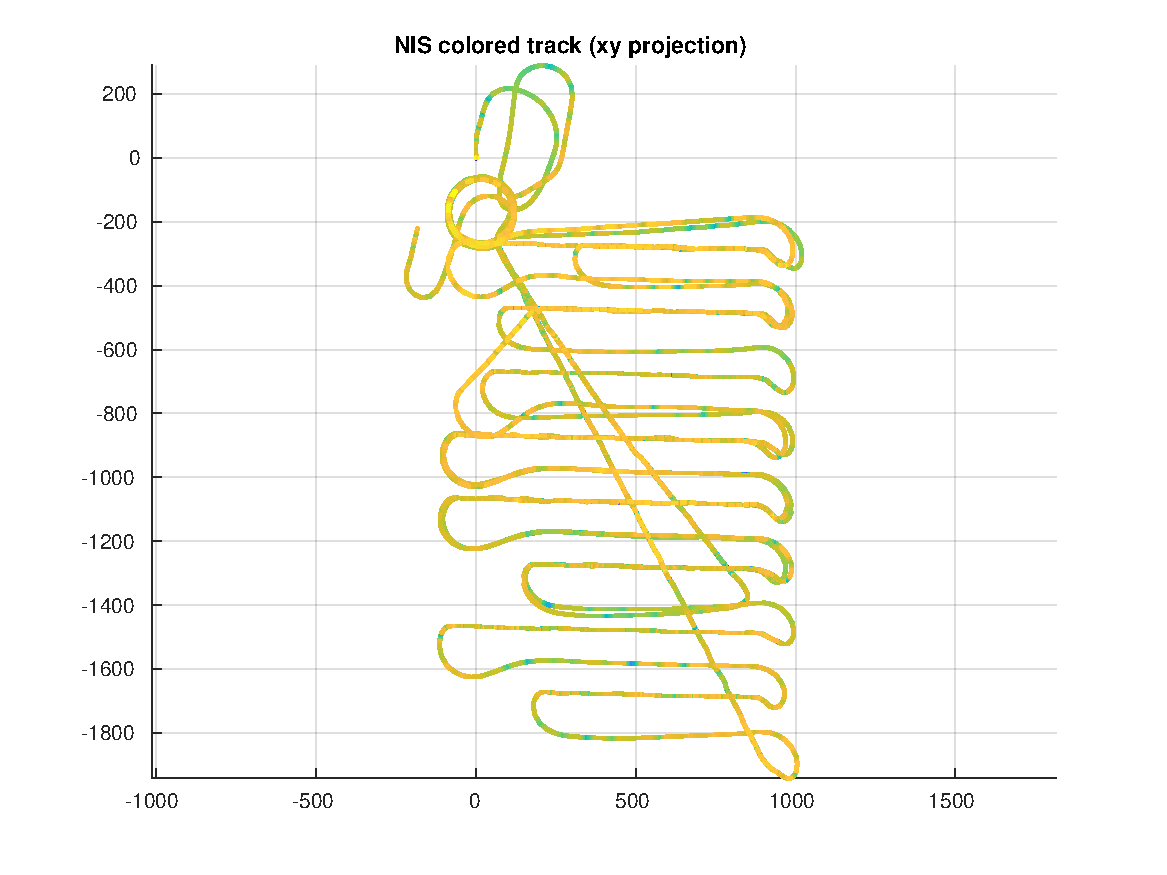
\includegraphics[width=\textwidth]{plots/a2-real-nis-colored-track}
                \caption{NIS colored track}
                \label{fig:eskf-real-nis-coloredtrack}
        \end{subfigure}
        \caption{ESKF NIS for the real dataset}
\end{figure}
\begin{figure}
        \begin{subfigure}[b]{0.49\textwidth}
                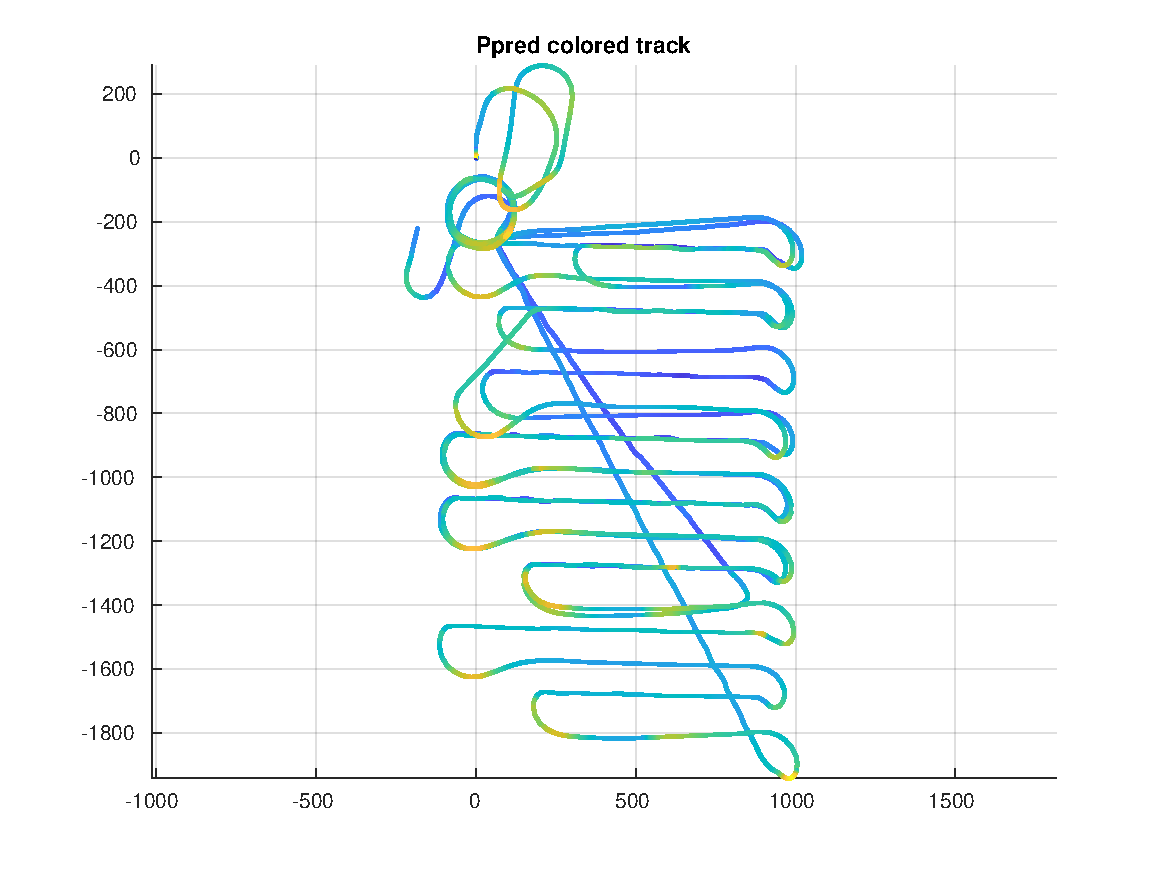
\includegraphics[width=\textwidth]{plots/a2-real-ppred-colored-track}
                \caption{$P_{pred}$ norm colored track}
                \label{fig:eskf-real-ppred-coloredtrack}
        \end{subfigure}
        \hfill
        \begin{subfigure}[b]{0.49\textwidth}
                \includegraphics[width=\textwidth]{plots/a2-real-track}
                \caption{UAV Track for the real dataset. Red=GNSS measurements, Blue=ESKF}
                \label{fig:eskf-real-track}
        \end{subfigure}
        \caption{ESKF results for the real dataset}
\end{figure}


\subsubsection{Discussion}

\subsubsection{Attitude estimation}
The attitude estimation for roll and pitch is very precise which makes sense since they are observable using the IMU due to the constant gravity vector. Yaw is however not possible to observe without additional requirements on the measurements. Without any sensor for measuring global heading (i.e compass) we need to get the heading from the planes velocity, which we can estimate from the GNSS measurements \textit{if the plane is moving.} If the velocity vector is zero, we have no information about the direction and can not estimate the heading. 

\




\section{}
\subsection{Introduction}
\subsubsection{The SLAM Problem}
In any autonomous manouvering situation, be it for a robot, a wheeled vehicle, a flying drone or anything in between, the need for localization is vital.
Localization alone however is only really meaningful in relation to the environment the robot is in.
The SLAM – simultaneous localization and mapping – problem arises then, as the need to simultaneously locate the robot as well as map out its environment.

This problem is naturally non-trivial and has consequently been the topic of extensive research in the last few decades.
There are multiple difficult aspects of the problem that must be solved for a SLAM-system to be successful.
Odometry, i.e. measuring the movement of the robot, map feature/landmark detection, data association as well as estimation and tracking are among the central parts of the SLAM problem that must all be solved.
One of the earliest SLAM solvers, which is the one we will be considering in this assignment is EKF-SLAM, in which an extended Kalman filter fuses together odometric measurements with associated landmark measurements to provide a continuously improved map of the environment and the vehicle position within it.

\subsubsection{EKF-SLAM in Intuitive Terms}
In our problem formulation, we are considering the odometry of the vehicle as given at each timestep, e.g. from an IMU or wheel encoders.
Using this information, typically in the form of velocity estimates or displacement increments, the vehicle can perform dead reckoning to give an indication of where the it has moved over time.
Such a scheme quickly breaks down however, as the inevitably imprecise odometric measurements, when integrated, will give rise to an ever accumulating deviation from the true position of the vehicle. In Kalman filter terms, this corresponds to performing consecutive prediction steps for all time. In order to remove deviations, the natural extension to this scheme is then to include an update step, where the pose, i.e. the position and orientation of the vehicle is updated with information gathered from observing the environment. In that sense, EKF-SLAM is similar to the ESKF, with landmark measurements replacing GNSS for global position updating.

\subsection{Our EKF-SLAM Implementation}
The problem we are considering in this assignment is two-dimensional SLAM, meaning the vehicle is modeled with three degrees of freedom, $x$, $y$ position and orientation $\psi$. In contrast, the ESFK in \ref{sec:a2} was able to represent 6 degrees of freedom. The other major difference is that the state vector in EKF-SLAM contains all the discovered landmarks. We call this state vector the joint pose-landmark vector $\eta_k = \begin{bmatrix} \mathbf{x}_k & \mathbf{m} \end{bmatrix}^{\top}$ as it contains both the pose and all landmarks detected up to the current timestep. In the predict step of the EKF, the pose is compounded (i.e. added in a geometrically meaningful way) with the current odometric vector $\mathbf{u}_k$, in addition to updating the covariance matrix. The update step however is where the action happens. During this step, the EKF does three things. Firstly, it associates new measurements with existing landmarks using Joint Compatibility Branch and Bound, or JCBB for short. Secondly, it calculates an innovation term from the associations that it does an Kalman update step with. Lastly, it augments the state vector with new landmarks – one for each unassociated measurement.

\subsubsection{Joint Compatibility Branch and Bound}
As mentioned, our implementation uses the JCBB algorithm for associating measurements with landmarks. The important feature of this algorithm is that is finds the best joint compatibility in addition to individual compatibility. For SLAM, joint compatibility is absolutely necessary as a set of individually compatible measurements can still be jointly incompatible and updating the Kalman filter with such an association can cause it to diverge.\cite{jcbb}



\subsection{Tuning of EKSF-SLAM for simulated dataset}
We started by tuning the odometry noise $Q$ and measurement noise $R$ by using NEES and NIS to get the initial tuning. We used a diagonal $Q$ and tuned the translation and heading independently to improve NEES. The measurement noise $R$ was tuned by attempting to maximize NIS while keeping the entries in $R$ as low as possible. We also created a plot for the position error over time to keep track of the estimation error. We realized that there were a tradeoff between a having a consistent filter (acceptable NIS and NEES) and the estimation error. Trying to improve the NEES resulted in increased error and trying to reduce the estimation error gave us worse NEES and NIS. We decided to prioritize the estimation error when tuning, but also kept an eye on the NEES and NIS to make sure we remained close to the confidene intervals. With our finished tuning we achieved a $82\%$ within NIS CI and $68\%$ within NEES CI, while also keeping the estimaion error reasonably low (less than $0.5m$). The JCBB alphas was choosen not to low to avoid making too many wrong associations. Otherwise it was tuned by balancing it with the other parameters while looking at NEES, NIS and estimation error. 

\subsection{Victoria Park Dataset}
The Victoria Park dataset is a classic dataset for 2D SLAM that has been analyzed numerous times in the literature. The dataset is generated by a car driving in Victoria Park, Sydney detecting trees with a front-mounted laser scanner and recording its odometry using encoders and steering sensors. When tuning for this dataset we initialized the filter with the standard deviations found using the simulated dataset. We used the same normalized NIS as we did in \cref{a3-sim-tuning} and tried to get as consistent results as possible by targeting the amount of NIS within our $95\% \chi^2$ CI. Due to the lack of ground truth, except for the highly unreliable GNSS data, we considered NEES to be unavailable. By considering the tracking error and NIS we tuned our filter to get as precise results as possible while still getting a somewhat consistent filter. We found that choosing $R$ too small resulted in more doubly registered landmarks, as the filter put too much trust in measurements. Our finished tuning resulted in $37\%$ within the NIS CI. Knowing however that the EKF has an issue with consistency for SLAM, we decided to focus on providing robust tracking with little deviation from the GNSS measurements instead of chasing a perfectly consistent filter. As can be seen in figures \ref{fig:a3-real-results_bg} and \ref{fig:a3-real-gnss-diff}, the tracking is satisfactory and deviates by at most 10 meters from the GNSS measurements. It should be noted that GNSS measurements cannot in general be regarded as a true ground truth. It is also aligned by hand in our case, further contributing to the error.
\begin{tcolorbox}[ams align, title={ESKF-SLAM tuning for Victoria Park dataset}]
    Q &= \begin{bmatrix}0.0016 & 0 & 0 \\0 & 0.0016 & 7.2*10^{-4} \\0 & 7.2*10^{-4} & 4*10^{-4} \end{bmatrix} & R &= \begin{bmatrix}0.01 & 0 \\0 & 0.01\end{bmatrix} \\
    \alpha_{1} &= 10^{-5} & \alpha_2 &= 10^{-3}
\end{tcolorbox}

\subsection{Discussion}
\subsubsection{Computational Performance of EKF-SLAM}
EKF-SLAM has been critizised for a variety of reasons in the literature, and one of the issues often brought up is computational performance as the map grows. Keeping the computation time down is of paramount importance in the online SLAM problem where delayed updates are not acceptable. In fact, each timestep of EKF-SLAM has a computational complexity of $\mathcal{O}(n^2)$ in the number of detected landmarks\cite{divideandconq}, something our implementation confirms. When tuned to provoke lots of landmark detections (around 800), the update step of the Kalman filter takes quadratic time, as shown in figure \ref{fig:update_time_landmarks}. These results show that in large environments, EKF-SLAM alone fails to meet the time-requirements for online SLAM.
\begin{figure}
    \centering
    \begin{subfigure}{0.45\textwidth}
        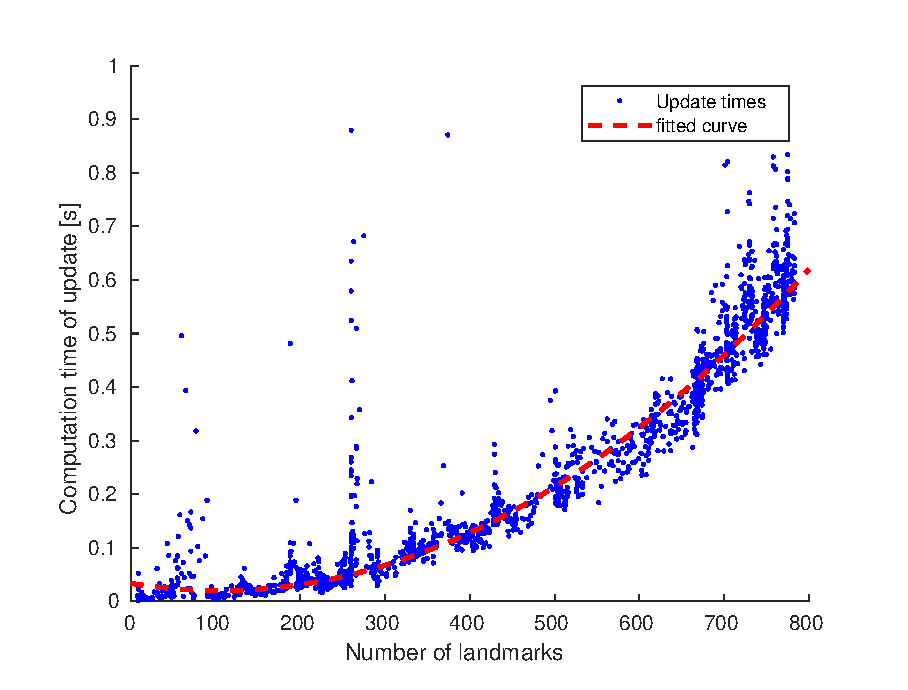
\includegraphics[width=\textwidth]{plots/a3/update-time-vs-landmarks}
        \caption{Update time vs landmarks}
        \label{fig:update_time_landmarks}
    \end{subfigure}%
~
    \begin{subfigure}{0.45\textwidth}
        \includegraphics[width=\textwidth]{plots/a3-real-results-bg}
        \caption{Trajectory overlayed Google Maps}
        \label{fig:results_bg}
    \end{subfigure}
\end{figure}

\subsubsection{Measurement Clutter}
After a successful run of the EKF-SLAM algorithm on the Victoria Park dataset, we typically find around 300 landmarks. For this reason, we have speculated that not all these landmarks correspond to actual trees, even though that is what they are supposed to represent. One of the reasons for this is landmarks being doubly registered due to the JCBB algorithm not making the proper associations. But another reason that must not be overlooked is the effect of clutter in the measurement data. The laser data in the dataset has been processed to only contain measurements that match a certain tree-profile\cite{victoria}, however no classification algorithm is perfect and we speculate that a lot of the measurements are spurious and should be regarded as clutter. This partly stems from the fact that a lot of the detected landmarks happen to appear inside the six-lane intersection to the east of Victoria Park, as can be seen in figure \ref{fig:results_bg}. In our experiments, the effect of clutter has not been significant, and spuriously detected landmarks have not had a noticeable impact on SLAM performance. It might however become problematic for longer operation times and larger maps. Keeping the number of landmarks down is essential to successfully apply EKF-SLAM in an online situation. In addition, wrongly registered landmarks might lead to spurious associations in the future and ultimately worsen the tracking performance.

\subsubsection{Choice of JCBB CI Bounds with Implication on Robustness}
The JCBB algorithm operates with two confidence intervals, one for joint and one for individual compatibility. The Mahalonobis distances of both joint and individual compatibility are gated with these confidence intervals to determin whether to move on with a given hypothesis.\cite{jcbb} In the Victoria Park dataset, we found that the choice of large confidence intervals ($\alpha_1 = 10^{-5}$ and $\alpha_2 = 10^{-3}$ for joint and individual respectively) gave perfectly satisfactory association speed on the dataset, however when EKF-SLAM was rerun on the generated map with a slight offset in orientation of $6^\circ$ (such a situation could appear naturally from disturbances such temporary loss of sensor data), the JCBB algorithm wound up in an almost complete stall after a few hundred timesteps, likely because all hypothesis were regarded as more equally likely due to the offset, making the algorithm unable to reduce the search tree and single out the best association in reasonable time. Choosing tighter confidence intervals on the other hand, with $\alpha = 0.1$ for both joint and individual, many more associations were gated out and hence only the most promising hypotheses were considered, ultimately leading to reasonable execution times. In the end, this made the rerun on the previously built map perfectly possible with no significant slow-down. This result shows how the choice of these confidence intervals is detrimental to the robustness of EKF-SLAM and crucial for online SLAM as a small disturbance can cause the JCBB algorithm to fail to find associations within reasonable time.




\printbibliography
\end{document}

